\scanpage{52}
\mspage{\unsure{6}}
Je vais introduire, dans la sphère $\widetilde\Sigma$ dont le degré de connexion est 0, cinq ouverts, pris aussi grands que possible, qui soient simplement connexes -- obtenus en pratiquant des ``coupures'' qui relient entre eux les \deleted{trois} bords $U_i$ des trois ``trous'' \deleted{$\unsure{\Sigma}$}. On pose
\figure{
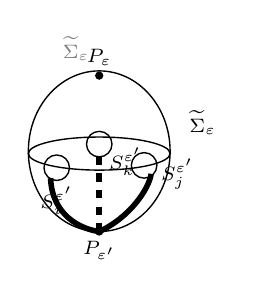
\begin{tikzpicture}[x=.6cm,y=.6cm,every node/.style={font=\scriptsize},line width=.5pt]
\draw (0,0) ellipse (1.5 and 1.7);
\draw (0,-.05) ellipse (1.5 and .35);
\draw (-.9,-.35) circle (.27); \draw (0,.15) circle (.27); \draw (.95,-.3) circle (.27);
\draw[line width=2pt] (-1.03,-.57) .. controls (-1,-1.35) and (-.4,-1.65) .. (0,-1.7) .. controls (.65,-1.4) and (1.05,-.8) .. (1.1,-.48);
\draw[line width=2pt,dashed] (0,-.12)--(0,-1.7);
\fill (0,1.6) circle (1.5pt); \fill (0,-1.7) circle (1.5pt);
\node[above] at (0,1.6) {$P_\varepsilon$}; \node[above left,gray] at (0,1.7) {$\widetilde\Sigma_\varepsilon$};
\node[below] at (0,-1.7) {$P_{\varepsilon'}$};
\node[right] at (0,-.22) {$S_k^{\varepsilon'}$}; \node[below] at (-.9,-.55) {$S_i^{\varepsilon'}$}; \node[right] at (1.1,-.48) {$S_j^{\varepsilon'}$};
\node[right] at (1.7,.6) {$\widetilde\Sigma_\varepsilon$};
\end{tikzpicture}
}
\[
(27)\quad\left\{\begin{aligned}
\widetilde\Sigma_\varepsilon&=\widetilde\Sigma\setminus\bigcup_{i\in J}\operatorname{supp}d_i^\varepsilon \qquad\varepsilon\in\uline{\varepsilon}\\
\widetilde\Sigma_i&=\widetilde\Sigma\setminus\bigcup_{\substack{j\in J\setminus\{i\}\\\deleted{\omega\in\uline{\omega}}}}\deleted{\operatorname{supp}}b_i^{\deleted{\unsure{\omega}}}
\end{aligned}\right.
\]
\margin{(où $b_i=\operatorname{supp}\widetilde b_i^\omega$\newline
\deleted{$=\operatorname{supp}\unsure{c_i^\omega|b_i^\omega}\cup\operatorname{supp}\unsure{c_i^{\omega'}|b_i^{\omega'}}$}\newline
$=\operatorname{supp}\unsure{c_i^\omega|b_i^\omega}\cup\operatorname{supp}\unsure{c_i^{\omega'}|b_i^{\omega'}}$)}
\figure{
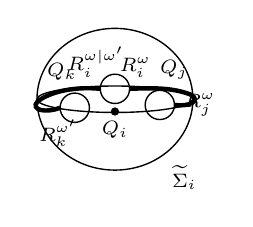
\begin{tikzpicture}[x=.6cm,y=.6cm,every node/.style={font=\scriptsize},line width=.5pt]
\draw (0,0) ellipse (1.65 and 1.5);
\draw (0,0) ellipse (1.65 and .28);
\draw (-.85,-.18) circle (.31); \draw (0,.22) circle (.31); \draw (.95,-.12) circle (.31);
\draw[line width=1.6pt] (-.31,.22) .. controls (-.8,.27) and (-1.35,.18) .. (-1.64,-.05) .. controls (-1.8,-.23) and (-1.45,-.3) .. (-1.16,-.18);
\draw[line width=1.6pt] (.31,.22) .. controls (.8,.24) and (1.2,.25) .. (1.6,.1) .. controls (1.85,-.03) and (1.55,-.17) .. (1.26,-.12);
\fill (0,-.26) circle (1.5pt); \node[below] at (0,-.26) {$Q_i$};
\node[above] at (-1.12,.2) {$Q_k$}; \node[above] at (1.25,.22) {$Q_j$};
\node[above] at (-.4,.25) {$R_i^{\unsure{\omega|\omega'}}$}; \node[above] at (.43,.25) {$R_i^\omega$};
\node[below] at (-1.2,-.22) {$\unsure{R_k^{\omega'}}$}; \node[right] at (1.26,-.12) {$R_j^\omega$};
\node[below right] at (1,-1.2) {$\widetilde\Sigma_i$};
\end{tikzpicture}
}
Ce sont bien des ouverts \deleted{\unsure{de }$\Sigma$} simplement connexes de la sphère à trous $\widetilde\Sigma$ (car les complémentaires \inserted{connexes et à} sont connexes. On dit que $P_\omega$ est le \uline{centre} de $\widetilde\Sigma_\omega$, $Q_i$ le \uline{centre} de $\widetilde\Sigma_i$.
\margin{ce sont des ouverts denses, et pour cette raison connexes.}
On pose
\[
(28)\quad\left\{\begin{aligned}
\Pi_\varepsilon&=\Pi_1(\widetilde\Sigma,\widetilde\Sigma_\varepsilon)\simeq\Pi_1(\Sigma^*,\Sigma_\varepsilon^*)\simeq\Pi_1(\Sigma^*,P_\varepsilon)\\
\Pi_i&=\Pi_1(\widetilde\Sigma,\widetilde\Sigma_i)=\Pi_1(\Sigma^*,\Sigma_i^*)\simeq\Pi_1(\Sigma^*,Q_i)
\end{aligned}\right.
\]
en faisant les identifications indiquées par ces formules. \deleted{\unsure{De}} Pour $\forall\ x\in\widetilde\Sigma_\omega$ resp. $x\in\widetilde\Sigma_i$, on pose
\[
(29)\quad\left\{\begin{aligned}
\varphi_{\varepsilon,x}\text{ ou }\varphi_\omega&:\Pi_\varepsilon\xrightarrow{\sim}\Pi_1(\widetilde\Sigma,x)\quad(\simeq\Pi_1(\Sigma^*,x)\text{ si }x\in\Sigma^*)\\
\text{\unsure{resp.}}\ \varphi_{i,x}\text{ ou }\varphi_i&:\Pi_i\xrightarrow{\sim}\Pi_1(\widetilde\Sigma,x)\qquad\text{--}
\end{aligned}\right.
\]
\margin{Les $\varphi$ sont appelés \uline{isom.} \uline{de} \uuline{\unsure{transition|trivialisation}}.}
\margin{51}
